% Comparison

\begin{slide}{Comparing IPC Methods}
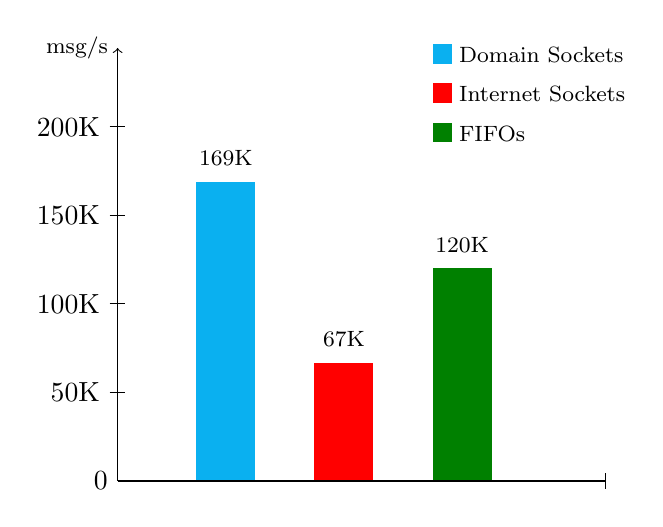
\begin{tikzpicture}

  % Domain Sockets
  \onslide<2->{
    \fill [ProcessBlue] (1, 0) rectangle ++(0.75, 3.8);
    \draw (1.375, 4.1) node {\footnotesize 169K};
  }

  % Internet Sockets
  \onslide<3->{
    \fill [Red] (2.5, 0) rectangle ++(0.75, 1.5);
    \draw (2.875, 1.8) node {\footnotesize 67K};
  }

  % FIFOs
  \onslide<4->{
    \fill [Green] (4, 0) rectangle ++(0.75, 2.7);
    \draw (4.375, 3) node {\footnotesize 120K};
  }

  % Legend
  \onslide<2->{
  \fill [ProcessBlue] (4, 5.3) rectangle ++(0.25, 0.25)
        node [pos=0.45, right, black]
        {\hspace{0.1cm}\footnotesize Domain Sockets};
  }

  \onslide<3->{
  \fill [Red] (4, 4.8) rectangle ++(0.25, 0.25)
        node [pos=0.45, right, black]
        {\hspace{0.1cm}\footnotesize Internet Sockets};
  }

  \onslide<4->{
  \fill [Green] (4, 4.3) rectangle ++(0.25, 0.25)
        node [pos=0.45, right, black]
        {\hspace{0.1cm}\footnotesize FIFOs};
  }

  % Axes (draw here to overdraw bar borders)
  \draw [-|] (0, 0) node [left] {0} -- (6.2, 0);
  \draw [->] (0, 0) -- (0, 5.5) node [left] {\footnotesize msg/s};

  % Ticks
  \foreach \y/\l in {1.125/50K, 2.25/100K, 3.375/150K, 4.5/200K} {
    \draw (-0.1, \y) node [left] {\l} -- ++(0.2, 0);
  }

  % \addplot[ybar, fill=Green] coordinates {(shared memory, 2217216)};
\end{tikzpicture}
\end{slide}

\begin{slide}{Comparing IPC Methods}
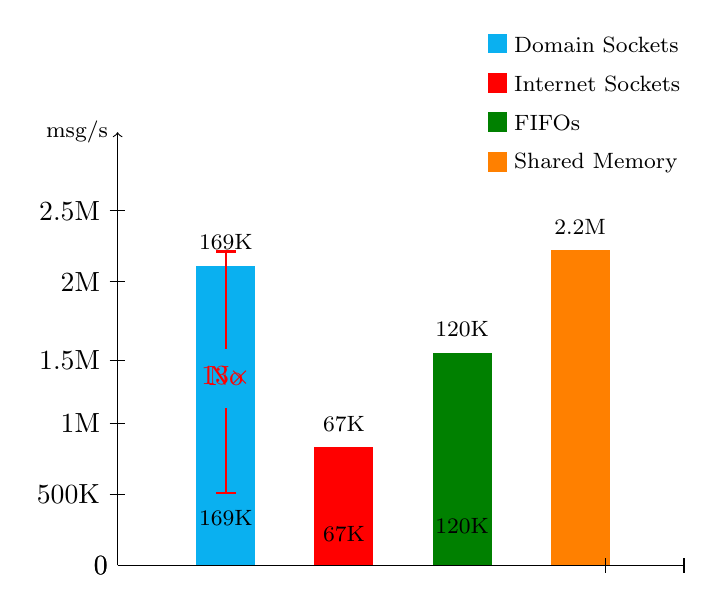
\begin{tikzpicture}

  % Domain Sockets
  \onslide<1>{
    \fill [ProcessBlue] (1, 0) rectangle ++(0.75, 3.8);
    \draw (1.375, 4.1) node {\footnotesize 169K};
  }
  \onslide<2->{
    \fill [ProcessBlue] (1, 0) rectangle ++(0.75, 0.3);
    \draw (1.375, 0.6) node {\footnotesize 169K};
  }

  % Internet Sockets
  \onslide<1>{
    \fill [Red] (2.5, 0) rectangle ++(0.75, 1.5);
    \draw (2.875, 1.8) node {\footnotesize 67K};
  }
  \onslide<2->{
    \fill [Red] (2.5, 0) rectangle ++(0.75, 0.1);
    \draw (2.875, 0.4) node {\footnotesize 67K};
  }

  % FIFOs
  \onslide<1>{
    \fill [Green] (4, 0) rectangle ++(0.75, 2.7);
    \draw (4.375, 3) node {\footnotesize 120K};
  }
  \onslide<2->{
    \fill [Green] (4, 0) rectangle ++(0.75, 0.2);
    \draw (4.375, 0.5) node {\footnotesize 120K};
  }

  % Shared Memory
  \onslide<3->{
    \fill [orange] (5.5, 0) rectangle ++(0.75, 4);
    \draw (5.875, 4.3) node {\footnotesize 2.2M};
  }

  % Legend
  \fill [ProcessBlue] (4.7, 6.5) rectangle ++(0.25, 0.25)
        node [pos=0.45, right, black]
        {\hspace{0.1cm}\footnotesize Domain Sockets};
  \fill [Red] (4.7, 6) rectangle ++(0.25, 0.25)
        node [pos=0.45, right, black]
        {\hspace{0.1cm}\footnotesize Internet Sockets};
  \fill [Green] (4.7, 5.5) rectangle ++(0.25, 0.25)
        node [pos=0.45, right, black]
        {\hspace{0.1cm}\footnotesize FIFOs};
  \onslide<3->{
  \fill [orange] (4.7, 5) rectangle ++(0.25, 0.25)
        node [pos=0.45, right, black]
        {\hspace{0.1cm}\footnotesize Shared Memory};
  }

  % Axes (draw here to overdraw bar borders)
  \onslide<-2>{
    \draw [-|] (0, 0) node [left] {0} -- (6.2, 0);
  }
  \onslide<3->{
    \draw [-|] (0, 0) node [left] {0} -- (7.2, 0);
  }
  \draw [->] (0, 0) -- (0, 5.5) node [left] {\footnotesize msg/s};

  \foreach \y/\l in {0.9/500K, 1.8/1M, 2.6/1.5M, 3.6/2M, 4.5/2.5M} {
    \draw (-0.1, \y) node [left] {\l} -- ++(0.2, 0);
  }

  % Factor
  \onslide<4>{
    \draw [red, thick, |-] (1.375, 0.9) -- (1.375, 2);
    \draw [red] (1.375, 2.4) node {13$\times$};
    \draw [red, thick, -|] (1.375, 2.75) -- (1.375, 4);
  }

  \onslide<5>{
    \draw [red, thick, |-] (1.375, 0.9) -- (1.375, 2);
    \draw [red] (1.375, 2.4) node {No};
    \draw [red, thick, -|] (1.375, 2.75) -- (1.375, 4);
  }
\end{tikzpicture}
\end{slide}
